\documentclass[a4paper,12pt,final]{article}


\usepackage{graphicx}
\title{
\begin{center}
  	
\includegraphics[scale=0.3]{101Logo.png} 
  \end{center}
  \textbf{\\}
CSIR - Distributed Application Manager\\
User Manual\\
}
\author{101 Solutions}

\begin{document}
\maketitle
\begin{center}
Version 0.3
\end{center}
\textbf{\\}
\textbf{\\}
\textbf{\\}
\textbf{\\}
\textbf{\\}
\textbf{\\}
\begin{center}
\begin{tabular}{|l|l|}
\hline
Francois Germishuizen & 11093618\\
\hline
Jaco Swanepoel & 11016354\\
\hline
Henko van Koesveld & 11009315\\
\hline
\end{tabular}
\end{center}
\thispagestyle{empty}
\newpage
\thispagestyle{empty}
\textbf{\large{Change Log}}
\vspace{6pt}\newline
\begin{tabular}{|l|l|l|l|}
\hline
\textbf{Date} & \textbf{Version} & \textbf{Description} & \textbf{Done by}\\
\hline
22 Oct & Version 0.1 & Document Created & Jaco\\
\hline
22 Oct & Version 0.2 & Added basic descriptions of all  & Jaco\\
&&the functions&\\
\hline
22 Oct & Version 0.3 & Added general glossary with extensions & Jaco\\
\hline
22 Oct & Version 0.4 & Added images and minor checks  & Henko\\
\hline
29 Oct & Version 0.5 & Added detailed sys info  & Francois\\
\hline
31 Oct & Version 0.6 & Added help section info  & Francois\\
\hline
\end{tabular}
\newpage
\tableofcontents
\thispagestyle{empty}
\newpage

\pagenumbering{arabic}
\section{Overview}
\subsection{Background}
The CSIR is actively developing a distributed simulation framework that ties
in with various other real systems and is used to exchange information
between them. The client has a number of configurations of this system
depending on the requirements of the client which can involve various
external applications as well.\\
\textbf{\\}
One of the issues the client has is to quickly distribute the latest build or
configuration files of their software over various computers that are needed
for an experiment. In some cases the same computers may be used for other
experiments which mean each of the computers may need to have various
builds and configuration options.\\
\textbf{\\}
Another issue they experience is the running, stopping and restarting of
the complete simulation. During a simulation it may be determined that
certain configuration options may need to be changed and distributed to the
affected machines, in which case either all or some components will need to
be restarted which can become tedious and time consuming.
\subsection{Business opportunity}
The goal of our project is to develop an application which is able to maintain
various build versions of the simulation framework and distribute these builds
to certain designated machines that may be required for an experiment. The
application will monitor system statistics of the various machines attached
to an experiment and will have the ability to execute applications on those
machines which will have different configuration options.\\
\textbf{\\}
The application will consist of a master and slave component where the
master is used to control the distribution of slaves. From the master one will
be able to start an experiment which will run the relevant applications on all
the necessary machines.


\newpage
\section{Purpose of this document}
This document is intended to assist users of the application, known as AppMan and AppManClient, with neccessary tasks.



\section{Server use}

\subsection{Start Server}
The server is started automatically, but after a manual stop can be restarted maually as follows:

\subsection{Stop Server}
The server can be stopped using this menu item:

\subsection{Set Port}
The port can be changed from the default, effect will be taken when the server is restarted via a stop then start. The process looks as follows:

\section{Build related}

\subsection{Add Build to AppMan (Master)}
A build can be added on the master as follows, all the info, except build description is compulsory.

\begin{itemize}
\item Either click file -> Add build or drag and drop a folder onto the form which will open the following window and just enter the required details for the build.
\end{itemize}
\begin{center}
  	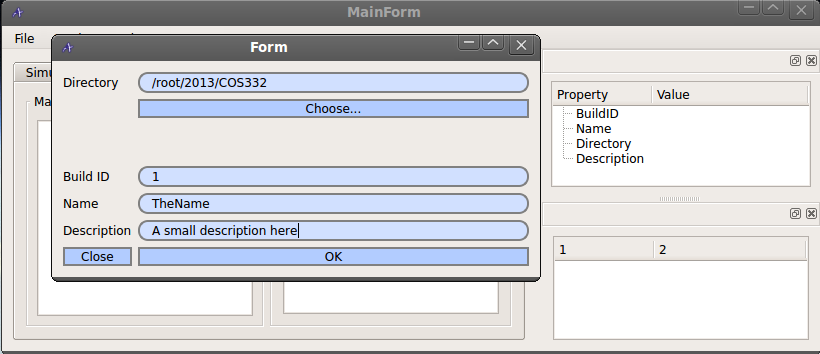
\includegraphics[scale=0.4]{AddBuildLinux.png}
 \end{center}

\subsection{Build syncrhonisation to AppManClient (Slave)}
The build can be copied in the following way:
\begin{itemize}
\item Double click the build you wish to copy over and then click copy over or go to file -> copy build over.
\item Enter the slave ip address you want to copy the file to
\end{itemize}

After a file changed in the build the changed files will automatically resynchronise after 25 seconds, but you can invoke it directly by:
\begin{itemize}
\item Double click the build you wish to resynch or click on the specefic machine where you want to resynch the build
\end{itemize}
 
 
Here is the menu where the build will resynchronise after 25 seconds and there is 5 seconds remaining. You can either click the resynch button to the right or directly under the build
\begin{center}
  	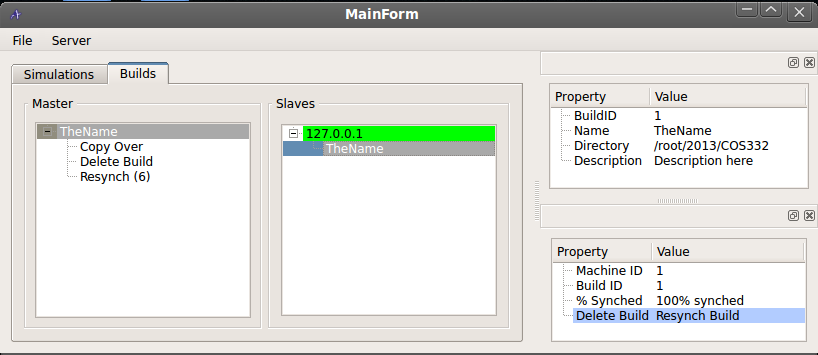
\includegraphics[scale=0.4]{5secResynch.png}
 \end{center}
 
 
Here is the menu of the build on the left hand side with the following options
\begin{itemize}
\item Copy Over

\item Delete Build
\item Resynch
\end{itemize}
\begin{center}
  	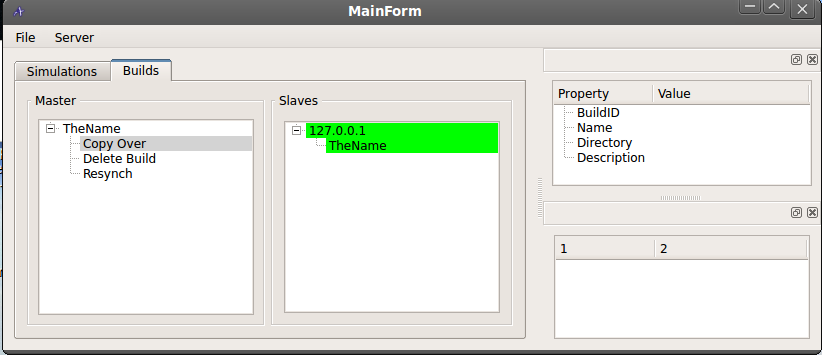
\includegraphics[scale=0.4]{MENU.png}
 \end{center}
 
 

\subsection{Build information editing}
You can edit the information for the build you just created.
\begin{itemize}
\item Click the build you want to edit
\item Double click the value on the right hand side as shown in the image below. The image below the description is edited. You are only able to change a small amount of things.
\end{itemize}
\begin{center}
  	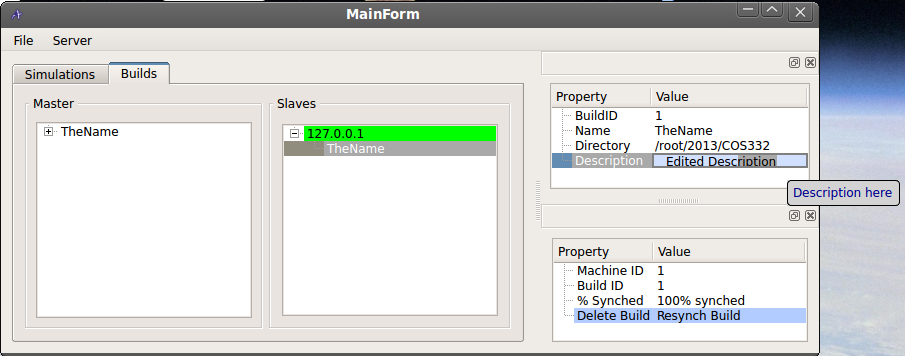
\includegraphics[scale=0.4]{EditedDescription.png}
 \end{center}


\section{Simulation related}

\subsection{Add Simulation}
To add a simulation one must have at least one slave added. The available slaves are displayed as checkbox items. A build or application can then be selected via a drop down box. If necessary command line arguments are then typed in. Once all the information is captured one can add the simulation. See below:

\begin{center}
  	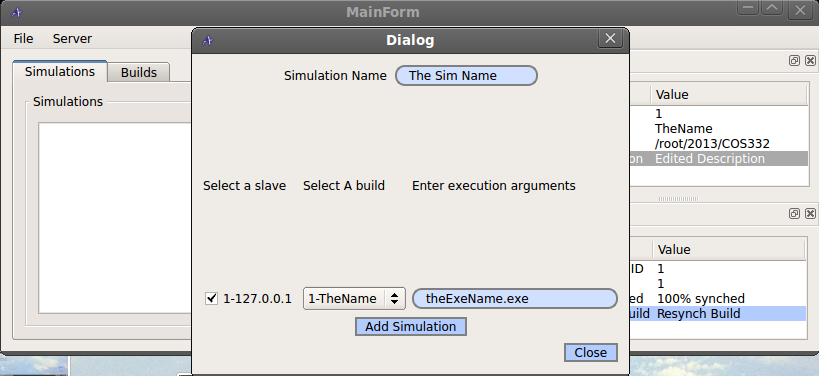
\includegraphics[scale=0.4]{AddSimFull.png}
 \end{center}

\subsection{Execute Simulation}
A simulation can be selected on the treewidget, then double-click the selected simulation. This will send the argument and required build or application name over the network, along with the command line arguments to the necessary slave. See below:

\begin{center}
  	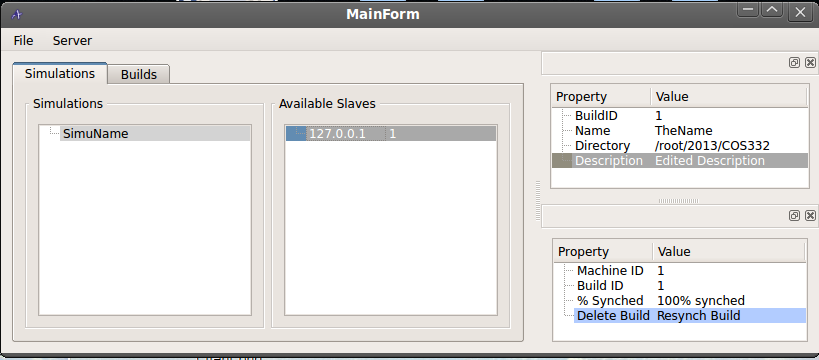
\includegraphics[scale=0.4]{ClickToRunSim.png}
 \end{center}

\section{Machine related}

\subsection{Connect}
On the AppManClient one sets the port and Master IP then clicks connect. These are then stored in a settings file for future use. 

\begin{center}
  	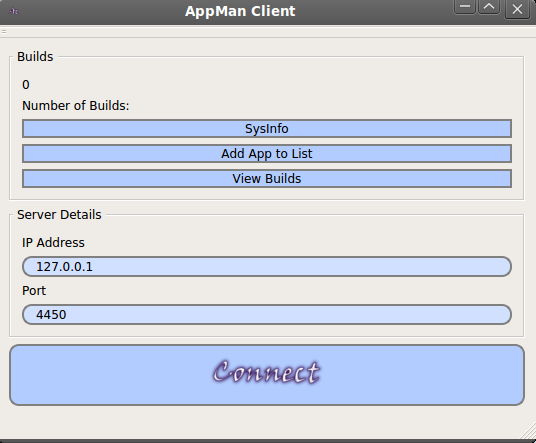
\includegraphics[scale=0.4]{InterfaceLinux_Client.png}
 \end{center}

\subsection{Request Minimal System Information}
When a slave is clicked the request is automatically sent to the slave, then displayed in a docking widget as follows (To the right hand side you can see the slave stats displayed).

\begin{center}
  	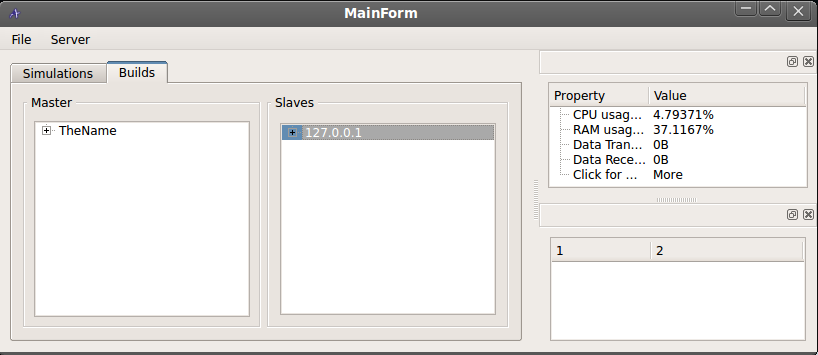
\includegraphics[scale=0.4]{SlaveStats.png}
 \end{center}
 
\subsection{Request Complete System Information}
After a slave is clicked to gain minimal system information the [Click for more...] button can be pressed to reveal much more detailed system information, such as a task list and disk drive information.

\begin{center}
  	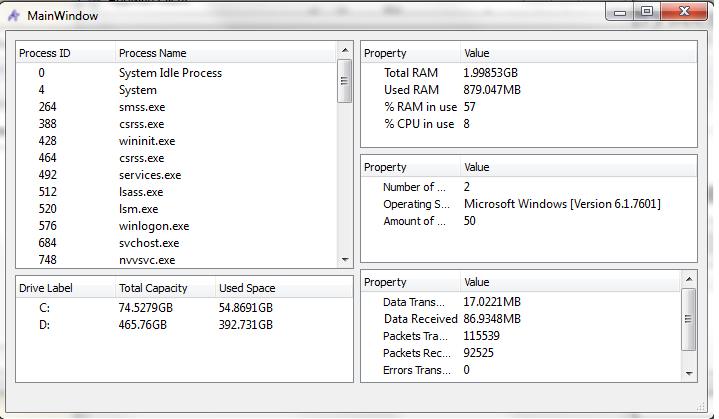
\includegraphics[scale=0.5]{DetSlaveStats.png}
 \end{center}
 
\section{Help section}
AppMan has a help section if any quick help is needed. It can be found by selecting the [About] menu option and then selecting [Help].  The help contains steps on doing most tasks relating to successful operation of AppMan.

\begin{center}
  	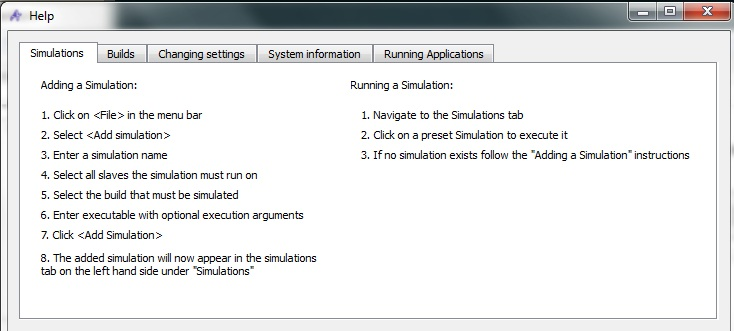
\includegraphics[scale=0.7]{AboutHelp.jpg}
 \end{center}

\newpage
\section{AppManClient}

\subsection{Add Application to AppList}
This is done for preinstalled programs and works by clicking the add app then it will go and add the app to the list of applications

\begin{center}
  	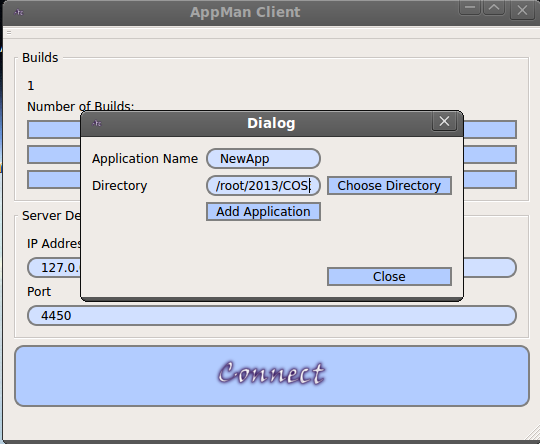
\includegraphics[scale=0.4]{AddAppToList.png}
 \end{center}
 
\subsection{View builds}
When the button is clicked, all builds and applications are displayed in a new window. See below:


\begin{center}
  	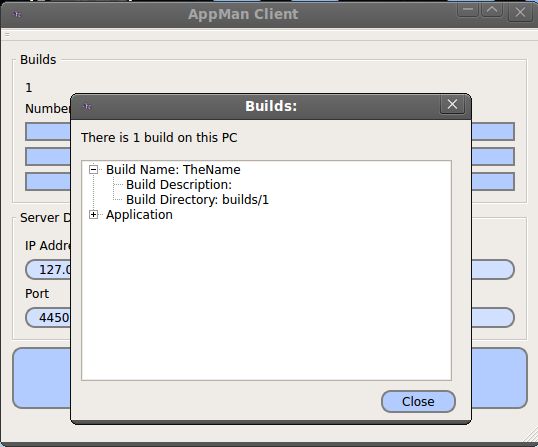
\includegraphics[scale=0.4]{SlaveBuilds.png}
 \end{center}


\newpage
\section{Glossary}
\begin{itemize}
\item{Build - An application build version that could potentially be distributed to slave computers.}
\item{Slave - A computer that will be controlled via a master computer. Application builds will be sent to this computer.}
\item{Master - A computer that will control Slaves across a network.}
\item{Server - A machine waiting on the network for connections from other machines.}
\item{GUI - Graphical User Interface with which a user can control the project.}
\item{Project - This project. The distributed application manager.}
\item{Application - A 3rd party program the client may use during simulations}
\end{itemize}

\end{document}